\section*{BACKGROUND}\label{s:background}
An effective interface to multiple robot programs is an important aspect to consider for a multi-robot applications simulation. The effort describes in this paper uses USARSim as a server allowing robot control programs (ROS)
to act as clients.

\subsection*{The USARSim Framework}
USARSim~\cite{CARPIN.LNAI.2006,WANG.WSC.2003} is a high-fidelity physics-based simulation system based on the industrial game engine Unreal Engine\footnote{http://www.unrealengine.com/}. USARSim was developed under a National Science Foundation grant to study Robot, Agent, Person Teams in Urban Search and Rescue~\cite{LEWIS.ICHC.2003}. Since Unreal
Engine has been deployed for the development of networked multi-player 3D
games, it solves many of the issues related to modeling, animation and rendering
of the virtual environment. Altogether, the Karma Physics
engine~\cite{KarmEngine} and high-quality 3D rendering facilities of the Unreal game engine allow the creation of realistic simulation environments that provide the embodiment of a robotic system. Furthermore, USARSim comes with tools to develop objects and environments (Unreal Editor) and it is possible to control actors in the game through a TCP/IP socket API.
%\begin{figure}[h!tbp]
%\centering \mbox{ \subfigure[]
%{\parbox{4.5cm}{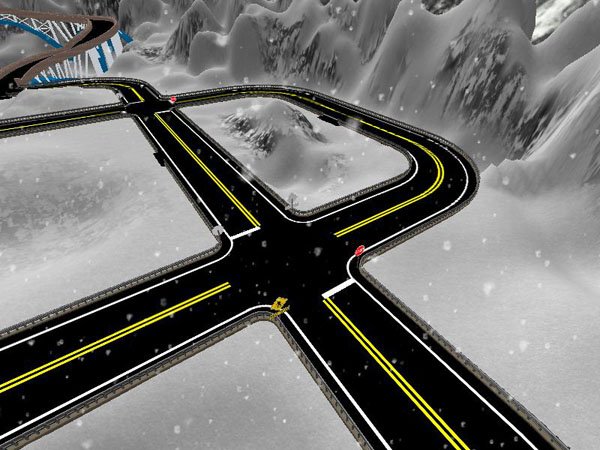
\psfig{file=arda1,width=4.5cm}}}} \quad
%\mbox{ \subfigure[] {\parbox{4.5cm
%}{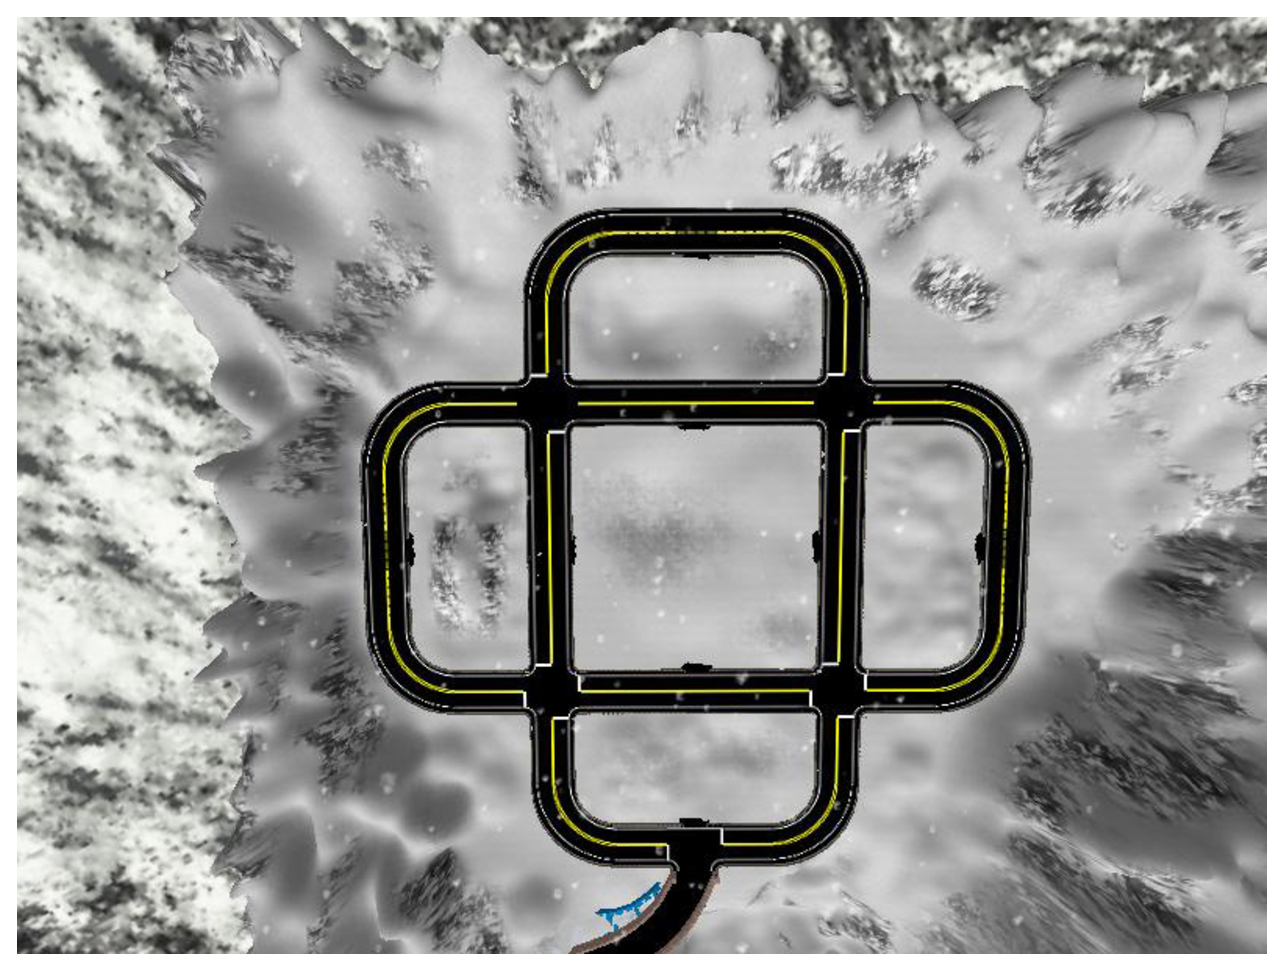
\psfig{file=arda4,width=4.5cm }}}}
%\caption{3D worlds in USARSim.} \label{usarsim}
%\end{figure}

%\begin{figure}[t]
%\begin{center}
%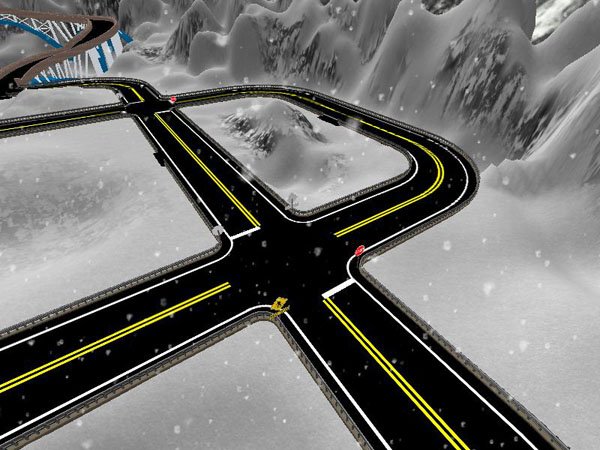
\includegraphics[scale=0.1]{arda1}
%\end{center}
%\caption{EXAMPLE OF VIRTUAL ENVIRONMENTS IN USARSIM.}
%\label{figure_ASME}
%\end{figure}

\subsection*{The ROS Framework}

ROS\footnote{http://www.ros.org/wiki/} is an open source framework designed to provide an abstraction layer to complex robotic hardware and software configurations. ROS delivers libraries and tools to help software developers create robot applications. ROS has been used in many robotic applications such as
Willow Garage\footnote{http://pr.willowgarage.com} Personal Robots Program~\cite{WYOBEK.ICRA.2008} and the Stanford University\footnote{http://stair.stanford.edu}
STAIR project~\cite{QUIGLEY.AAAI.2007}.


ROS possesses a large range of tools and services that both users and developers alike can benefit from. The philosophical goals of ROS include an advanced set of criteria and can be summarized as: peer-to-peer, tools-based, multi-lingual, thin, and free and open-source~\cite{QUIGLEY.ICRA.2009}. Furthermore, debugging at all levels of the software is made possible with the full source code of ROS being publicly available. Thus, the main developers of a project could benefit from the community and vice-versa.

\subsubsection*{Nomenclature}

The fundamental concepts of the ROS implementation are
nodes, messages, topics, and services. These terms will be used throughout the rest of the paper and are detailed below~\cite{QUIGLEY.ICRA.2009}.
\begin{itemize}
\item[-] Node: An executable unit which communicates with other nodes. ROS is
designed to be modular at a fine-grained scale: a system
is typically comprised of many nodes. In this context, the
term ``node" is interchangeable with ``software module". Nodes communicate with each other by passing messages.
\item[-] Message: A strictly typed data structure. Standard
primitive types (integer, floating point, boolean, \ldots) are
supported, as are arrays of primitive types and constants. A node sends a message by publishing it to a given topic.
\item[-] Topic: A communication channel between two or more
nodes. A node that is interested in a certain kind of data will subscribe
to the appropriate topic. There may be multiple concurrent
publishers and subscribers for a single topic, and a single
node may publish and/or subscribe to multiple topics.
\item[-] Service: A remote procedure call defined by a string name and a pair
of strictly typed messages: one for the request and one for
the response.
\end{itemize}